The Component Diagram shown below describes the logical components of the system we are to develop, from a very high-level description on to a more detailed one. This diagram does not take into account the deployment phase, hence it doesn’t describe the logical layer of the system in terms of the physical tiers where it is deployed.

\begin{figure}[H]
		\centering
		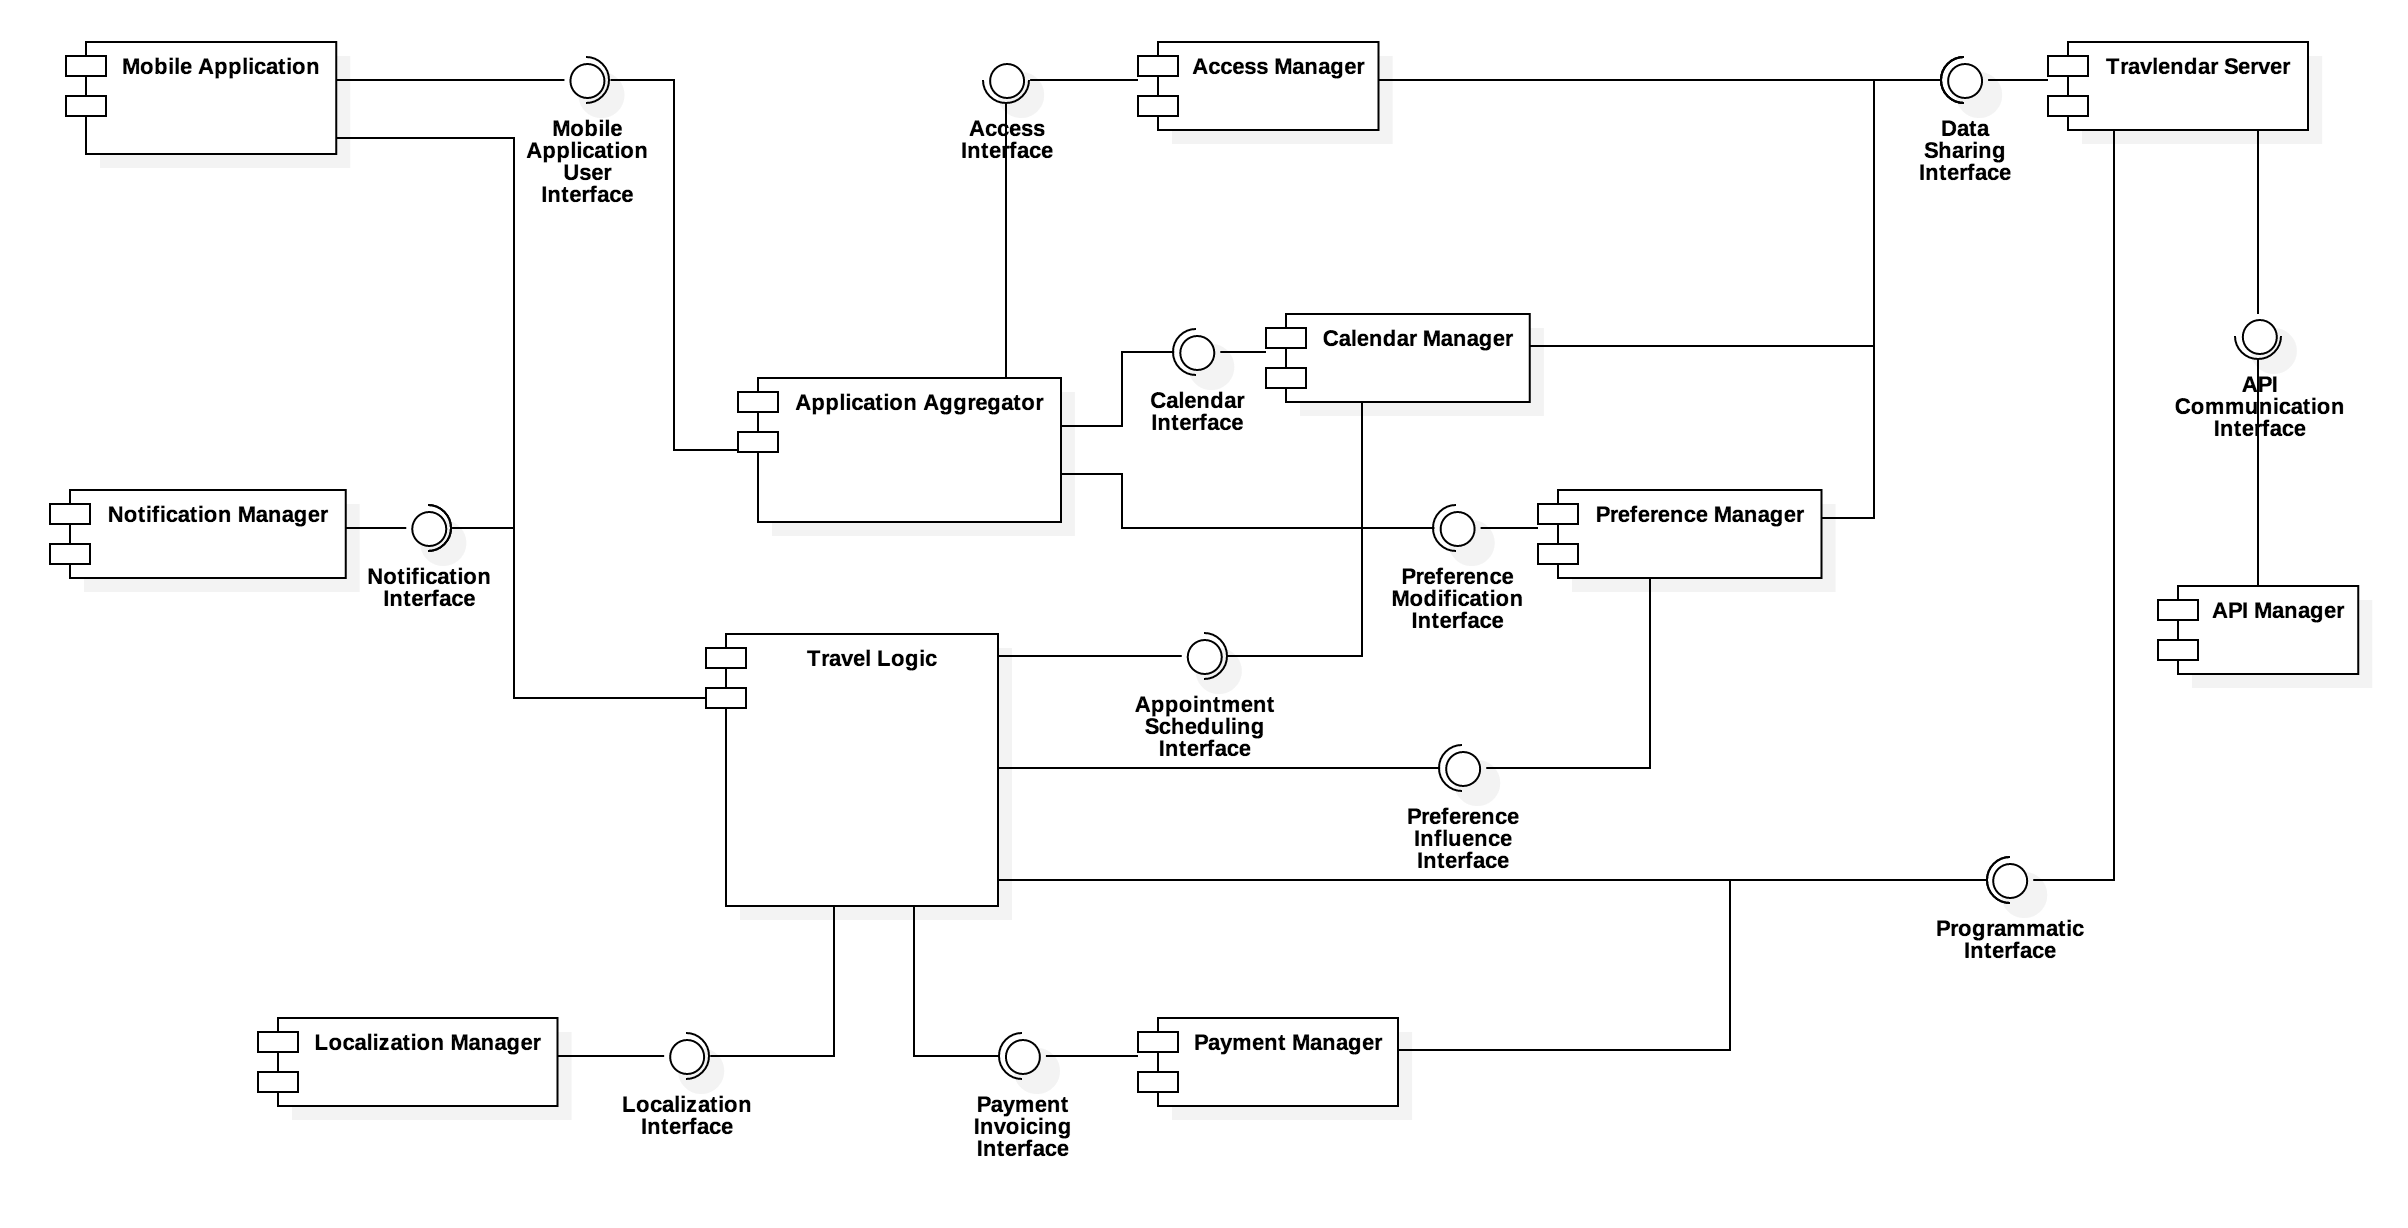
\includegraphics[width = \textwidth]{UML/componentDiagrams/highLevel}
		\caption{High level view}
		\label{componentHighLevel}
	\end{figure}

\paragraph{Mobile Application}
	This component represents the view of the User over its system. It’s split in two sub-components, Guest-view and User-view, which represents the two different ways an human interaction can be instaurated with the system.

	\begin{figure}[H]
		\centering
		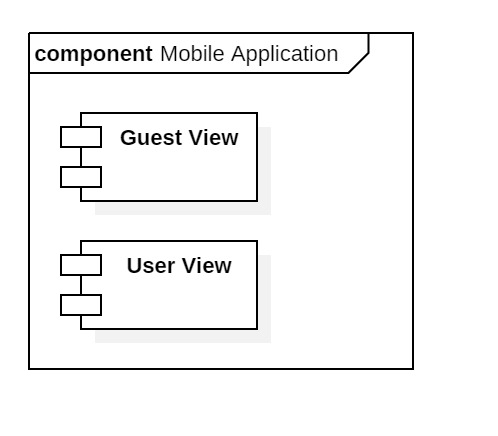
\includegraphics[scale = 0.2]{UML/componentDiagrams/mobileApplication}
	\end{figure}


\paragraph{Application Aggregator}
	This component works, unsuprisingly, as a collector of the different information \textit{Travlendar+} manages. It allows an easy management of every piece of information and allows us to avoid an high number of interfaces among the different components. 'Profile Manager' specifies the profile setting of the current user, while 'User Action Handler' allows us to register User's input.
	
	\begin{figure}[H]
		\centering
		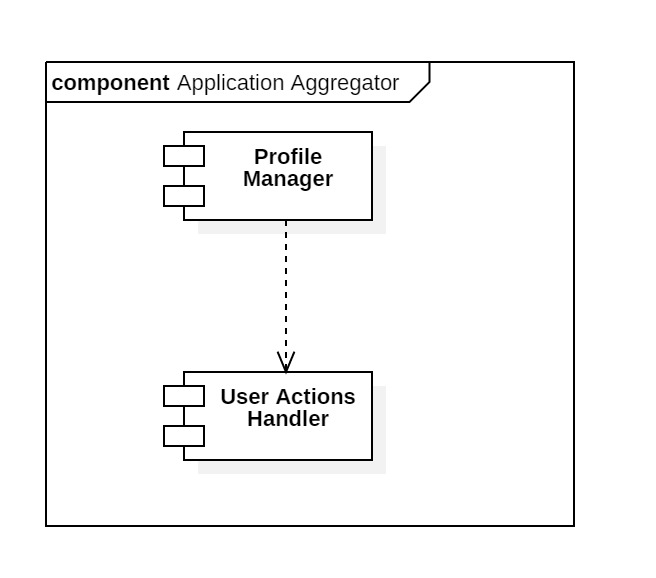
\includegraphics[scale = 0.2]{UML/componentDiagrams/applicationAggregator}
	\end{figure}
 
\paragraph{Calendar Manager}
	This component is divided into 'Appointments' and 'Breaks' sub-components, which track the appointments inserted by the User together with his breaks, and 'Trips', which is the list of trips arranged by the scheduler for every appointment. The sub-component 'Appointment Aggregator' serves the purpose of listing and presenting the content of the other two sub-components.
	
	\begin{figure}[H]
		\centering
		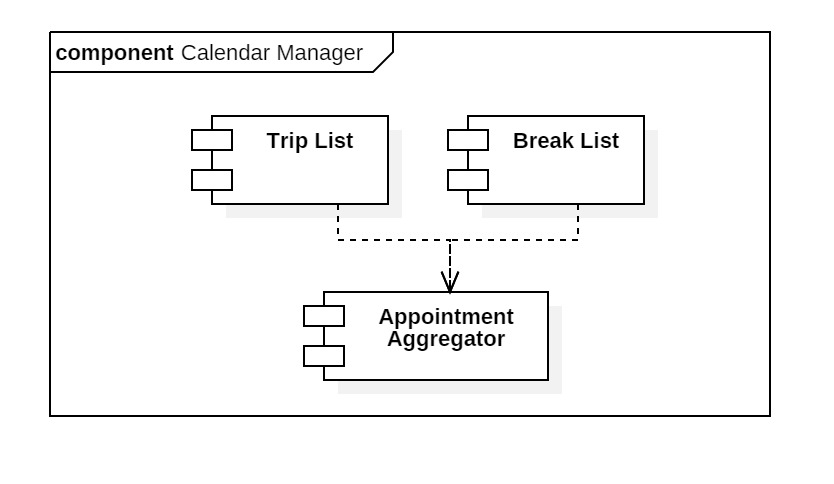
\includegraphics[scale = 0.2]{UML/componentDiagrams/calendarManager}
	\end{figure}
 

\paragraph{Preference Manager}
	This component serves the purpose of keeping track of the preferences expressed by the User. 'Season Pass Handler' takes care of storing season passes; 'Excluded Vehicles List' cuts off from the scheduler results involving a selection of banned transportation means, 'Preferences List' covers the remaining and wider spectrum of User's choices. 'Preference Handler' is the sub-component that manages the other ones and that communicates outside Preference Manager.

	\begin{figure}[H]
		\centering
		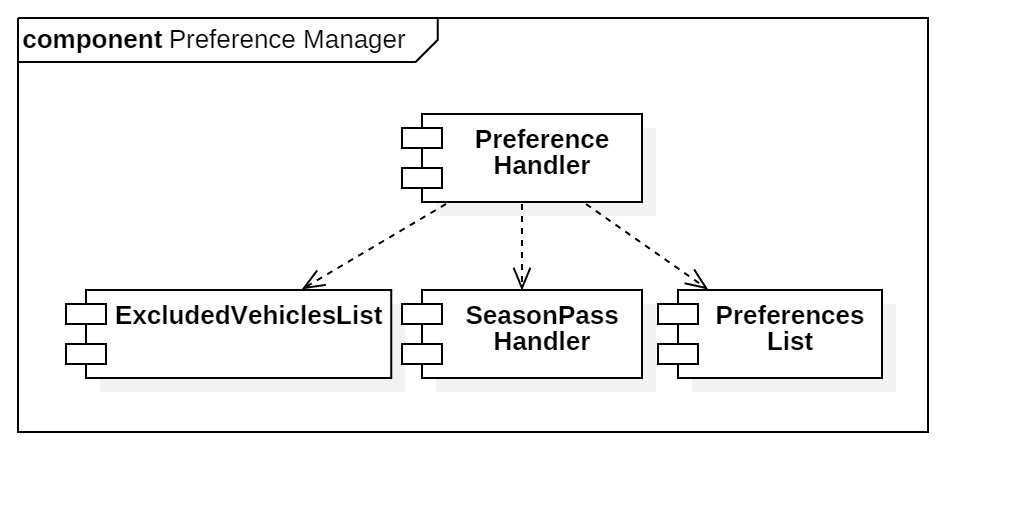
\includegraphics[scale = 0.2]{UML/componentDiagrams/preferenceManager}
	\end{figure}
	

\paragraph{Travlendar Server} 
	This component represents the \textit{Travlendar Server} whose purpose is to store User's preferences, access data and personal information. It is modeled by its 'DBMS' component, which stores Timetables and Preferences and the 'API Request Dispatcher', which forwards requests to external agents.

	\begin{figure}[H]
		\centering
		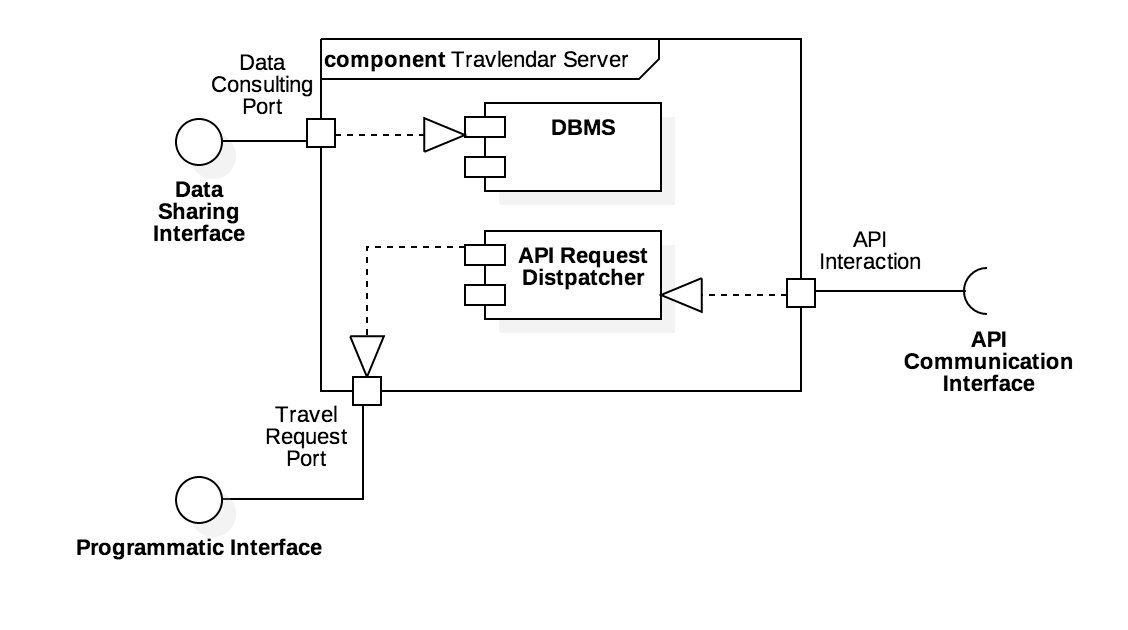
\includegraphics[scale = 0.2]{UML/componentDiagrams/travlendarServer}
	\end{figure}
	

\paragraph{Travel Logic Manager}
	This component is split into two sub-components: 'Scheduler' is the fundamental block that aims at scheduling and arranging User appointments and breaks via the the corresponding trips, 'DistanceManager' is the block whose purpose is to organize and present travel times to the scheduler in order to have them sorted out and well-managed.

	\begin{figure}[H]
		\centering
		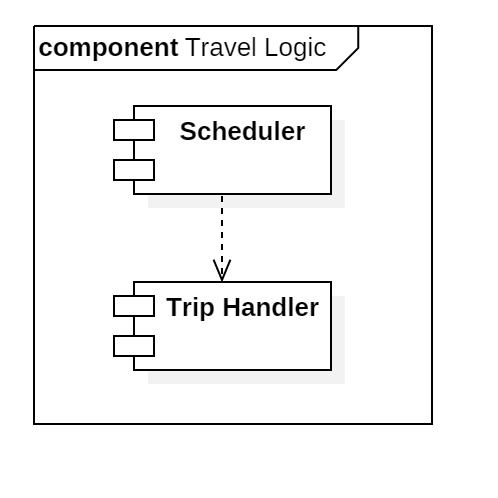
\includegraphics[scale = 0.2]{UML/componentDiagrams/travelLogic}
	\end{figure}
	

\paragraph{Payment Manager}
	This component deals with the recording of purchases and their associated credit cards.
	The sub-component 'Payment Handler' tracks purchase records and interacts with the required apps installed on the mobile device, while 'Purchase History' is an exploitable and rational organizations of the credit cards used by the user.

	\begin{figure}[H]
		\centering
		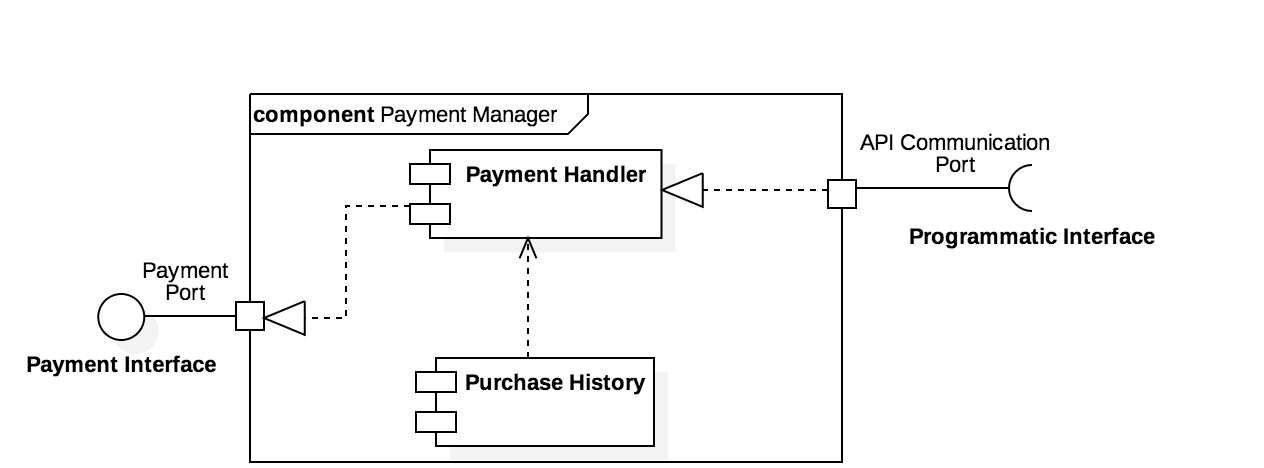
\includegraphics[scale = 0.2]{UML/componentDiagrams/paymentManager}
	\end{figure}
	

\paragraph{API Manager} 
	This component is critical in order to provide a functioning Travel Logic: it gathers the interactions with all external APIs.
	Here are listed the APIs the mobile application project starts with : Google Maps API, Google Transit API, Open Weather Map API, Car2Go and BikeMi API.
	The last couple is for reference only, as already pointed in the RASD. Naturally, the list of external services can be expanded.
	The 'Listener' component serves the purpose of forwarding requests and receives the desired inputs.
	
	\begin{figure}[H]
		\centering
		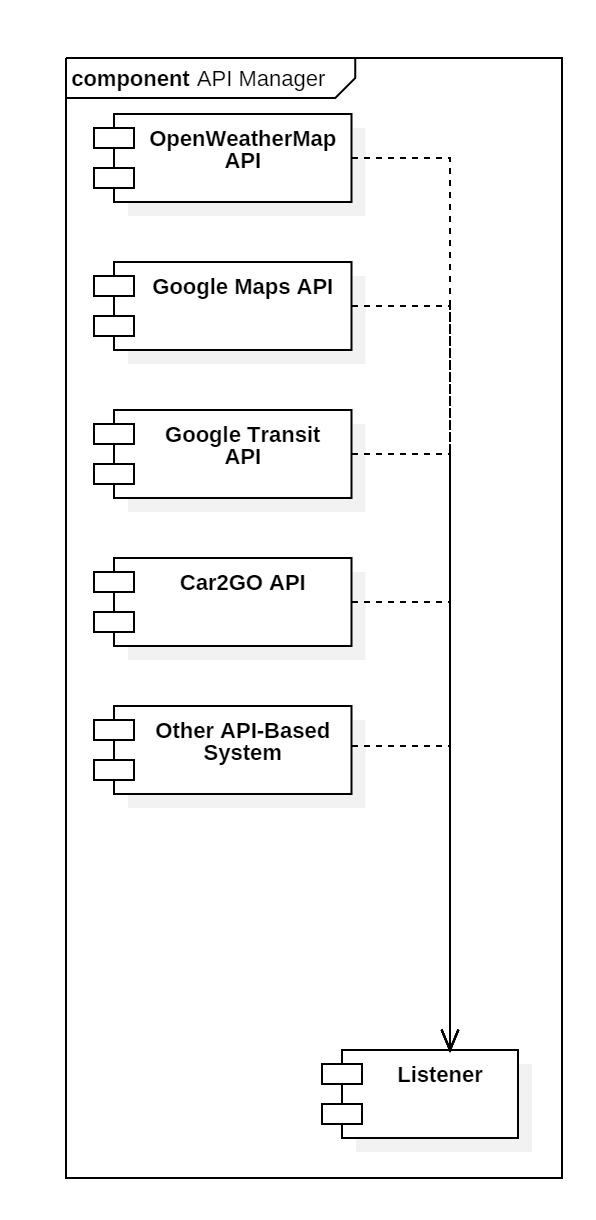
\includegraphics[scale = 0.2]{UML/componentDiagrams/APIManager}
	\end{figure}
	
	
\paragraph{Notification Manager}
	This component allows the notification system to warn users in the cases events partially or completely overlap according to the scheduler.

\paragraph{Localization Manager}
	This component represents the localization functionalities of the mobile application.
	
\begin{landscape}
	\begin{figure}
		\centering
		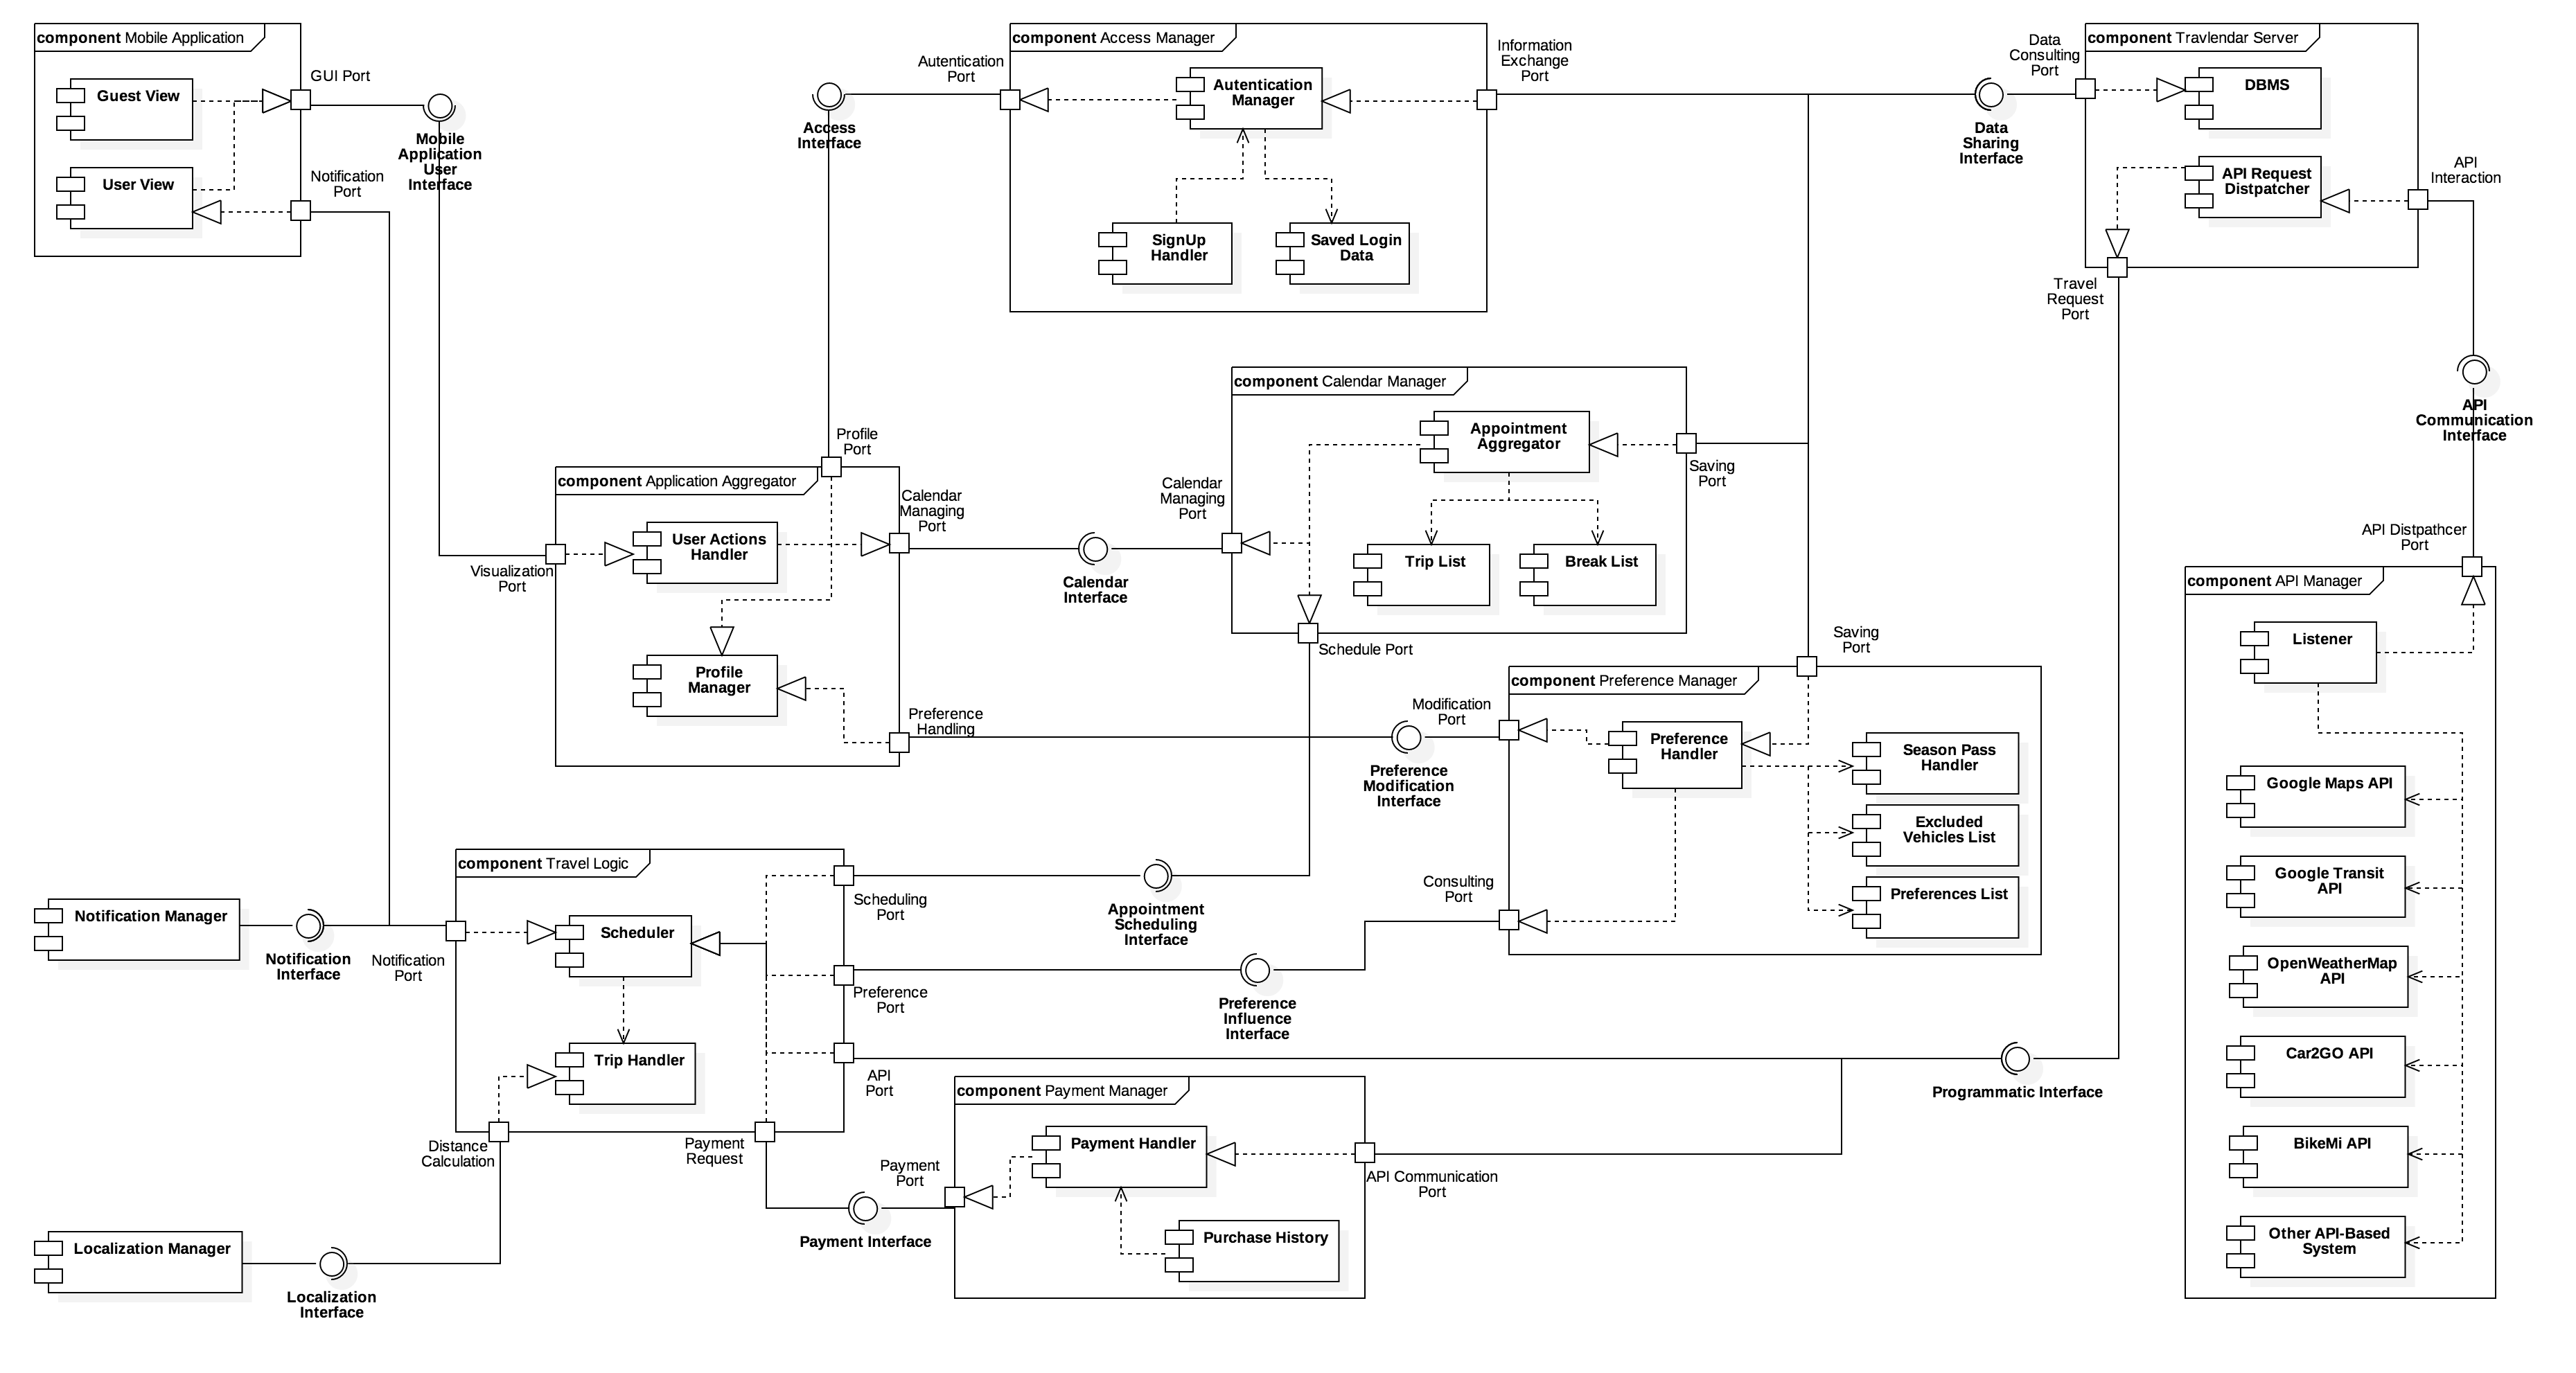
\includegraphics[height= 0.9\textheight]{UML/componentDiagrams/detailedLevel}
		\caption{Detailed level view}
		\label{detailedHighLevel}
	\end{figure}
\end{landscape}




